% !TEX TS-program = pdflatex
% !TEX encoding = UTF-8 Unicode

% This is a simple template for a LaTeX document using the "article" class.
% See "book", "report", "letter" for other types of document.

\documentclass[11pt]{article} % use larger type; default would be 10pt

\usepackage[utf8]{inputenc} % set input encoding (not needed with XeLaTeX)

%%% Examples of Article customizations
% These packages are optional, depending whether you want the features they provide.
% See the LaTeX Companion or other references for full information.

%%% PAGE DIMENSIONS
\usepackage{geometry} % to change the page dimensions
\geometry{a4paper} % or letterpaper (US) or a5paper or....
% \geometry{margins=2in} % for example, change the margins to 2 inches all round
% \geometry{landscape} % set up the page for landscape
%   read geometry.pdf for detailed page layout information

\usepackage[dvipdfmx]{graphicx} % support the \includegraphics command and options

% \usepackage[parfill]{parskip} % Activate to begin paragraphs with an empty line rather than an indent

%%% PACKAGES
\usepackage{booktabs} % for much better looking tables
\usepackage{array} % for better arrays (eg matrices) in maths
\usepackage{paralist} % very flexible & customisable lists (eg. enumerate/itemize, etc.)
\usepackage{verbatim} % adds environment for commenting out blocks of text & for better verbatim
\usepackage{subfig} % make it possible to include more than one captioned figure/table in a single float
% These packages are all incorporated in the memoir class to one degree or another...

%%% HEADERS & FOOTERS
\usepackage{fancyhdr} % This should be set AFTER setting up the page geometry
\pagestyle{fancy} % options: empty , plain , fancy
\renewcommand{\headrulewidth}{0pt} % customise the layout...
\lhead{}\chead{}\rhead{}
\lfoot{}\cfoot{\thepage}\rfoot{}

%%% SECTION TITLE APPEARANCE
\usepackage{sectsty}
\allsectionsfont{\sffamily\mdseries\upshape} % (See the fntguide.pdf for font help)
% (This matches ConTeXt defaults)

%%% ToC (table of contents) APPEARANCE
\usepackage[nottoc,notlof,notlot]{tocbibind} % Put the bibliography in the ToC
\usepackage[titles,subfigure]{tocloft} % Alter the style of the Table of Contents
\renewcommand{\cftsecfont}{\rmfamily\mdseries\upshape}
\renewcommand{\cftsecpagefont}{\rmfamily\mdseries\upshape} % No bold!

%%% END Article customizations

%%% The "real" document content comes below...

\title{極配置法}
\author{安齋智紀}
%\date{} % Activate to display a given date or no date (if empty),
         % otherwise the current date is printed 

\begin{document}
\maketitle

\section{2重極配置}
質量$m$の質点をPD制御($K_P, K_D$)で動かす.力の飽和は考えない.Fig. 1を参照.
\subsection{フィルタなし}
系の伝達関数を求める.目標値(入力)を$r$,現在の値(出力)を$x$とする.それぞれラプラス変換した後の値は$R(s), X(s)$とする.
\begin{eqnarray}
	(R-X)(K_P + K_D s) \frac{1}{ms^2} &=& X \\
	R-X &=& \frac{ms^2}{K_P + K_D s} X \\
	R &=& \frac{K_P + K_D s + ms^2}{K_P + K_D s} X \\
	G(s) &=& \frac{X}{R} = \frac{K_D s + K_P}{ms^2 + K_D s + K_P}
\end{eqnarray}
伝達関数$G(s)$の極はその分母の根である.それを負の実数の重解にすればよいから,各ゲインを
\begin{eqnarray}
	ms^2 + K_D s + K_P = m(s+\omega)^2 = ms^2 + 2ms\omega + m\omega^2 \\
   K_D = 2m\omega, \ K_P = m\omega^2 \ (\omega > 0)
\end{eqnarray}
と設計すれば,伝達関数は
\begin{eqnarray}
	G(s) &=& \frac{K_D s + K_P}{ms^2 + K_D s + K_P} \\
			 &=& \frac{2m\omega s + m\omega^2}{ms^2 + 2m\omega s + m\omega^2} \\
         &=& \frac{\omega^2 + 2\omega s}{(s + \omega)^2}                   
\end{eqnarray}
となる.

\subsection{フィルタあり}
フィルタなしのバージョンの伝達関数にステップ応答を与えるとオーバーシュートし,さらに分子の$s$があるせいでステップを入れた瞬間に入力が無限大に発散するという問題がある.そこでこの分子の項を打ち消すフィルタを設けてオーバーシュートせず収束する系を設計する.設計したい伝達関数は
\begin{equation}
	G(s) = \frac{\omega^2}{(s+\omega)^2}
\end{equation}
であるから,フィルタは
\begin{equation}
	G_F(s) = \frac{\omega^2}{\omega^2 + 2\omega s} = \frac{\omega}{\omega + 2s} = \frac{1}{1 + \frac{2}{\omega}s}
\end{equation}
と設計できる.これは時定数$\frac{2}{\omega}$のLPFである.このフィルタを入力$R$にかけることでこの伝達関数を設計できる(目標値との誤差$R-X$にかけるのではない).なぜなら,
\begin{eqnarray}
	G(s) = \frac{X(s)}{R(s)} G_F(s)^{-1} = \frac{X(s)}{R(s)G_F(s)} 
\end{eqnarray}
だからである.

\section{三重極配置}
考え方は二重極配置と特に変わらない.これにI制御を追加する.
\subsection{フィルタなし}
系の伝達関数は
\begin{eqnarray}
	(R-X)(\frac{K_I}{s} + K_P + K_D s) \frac{1}{ms^2} &=& X \\
	R-X &=& \frac{ms^2}{\frac{K_I}{s} + K_P + K_D s} X \\
	R &=& \frac{\frac{K_I}{s} + K_P + K_D s + ms^2}{\frac{K_I}{s} + K_P + K_D s} X \\
	G(s) &=& \frac{X}{R} = \frac{K_D s^2 + K_P s + K_D}{ms^3 + K_D s^2 + K_P s + K_I}
\end{eqnarray}
各ゲインを
\begin{eqnarray}
	ms^3 + K_D s^2 + K_P s + K_I = m(s+\omega)^3 = ms^3 + 3ms^2\omega + 3ms\omega^2 + m\omega^3 \\
   K_D = 3m\omega, \ K_P = 3m\omega^2, \ K_I = m\omega^3 \ (\omega > 0)
\end{eqnarray}
と設計すれば,伝達関数は
\begin{eqnarray}
	G(s) &=& \frac{K_D s^2 + K_P s + K_D}{ms^3 + K_D s^2 + K_P s + K_I} \\
			 &=& \frac{3m\omega s^2 + 3m\omega^2 s + 3m\omega}{ms^3 + 3m\omega s^2 + 3m\omega^2 s + m\omega^3} \\
         &=& \frac{\omega s^2 + 3\omega^2 s + 3\omega}{(s + \omega)^3}                   
\end{eqnarray}
となる.

\subsection{フィルタあり}
二重極配置と同じでこのままの伝達関数では必ずオーバーシュートするので分子を打ち消すフィルタを入れることを考える.フィルタの伝達関数は

\begin{equation}
	G_F(s) = \frac{\omega^3}{\omega s^2 + 3\omega^2 s + 3\omega} = \frac{\omega^2}{s^2 + 3\omega s + 3}
\end{equation}
である.

\begin{figure}[t]                                                                       
  \begin{center}                                                                        
    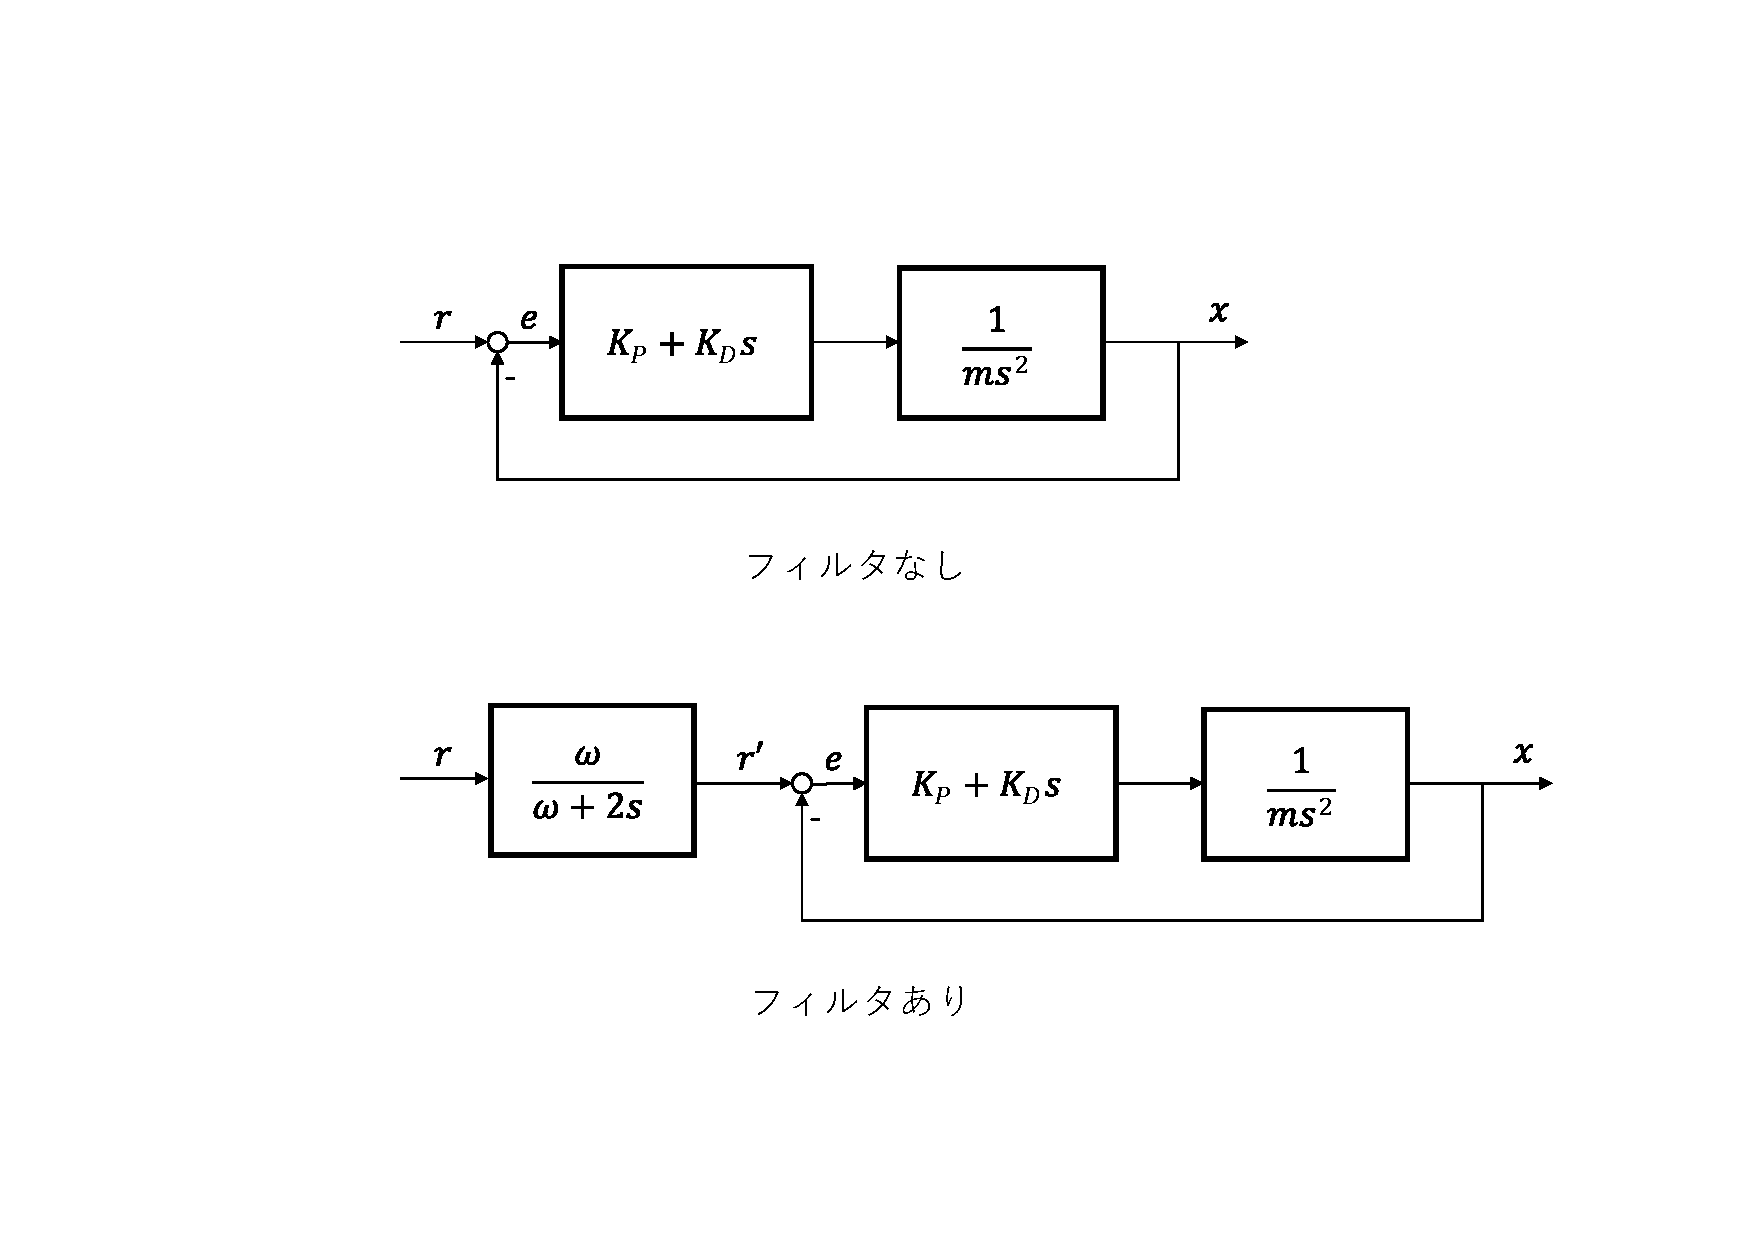
\includegraphics[width=1.0\columnwidth]{image.pdf}                        
  \end{center}                                                                          
  \caption{\label{figure:system}}          
\end{figure}

\end{document}
